\documentclass{beamer}

\usepackage{amsmath}
\usepackage{textcomp}
\usepackage{listings}
\usepackage{lmodern}
\usepackage{hyperref}
\usepackage[T1]{fontenc}


\lstset{
    language=[latex]tex,
    breaklines=true}

\usetheme{Madrid}

\setbeamertemplate{caption}{\raggedright\insertcaption\par}

\title[Committee Meeting 1]{First Committee Meeting}
\subtitle{Progress Report}
\author{Jason Balaci}

\institute{McMaster University}
\date{Oct. $21^{st}$, 2021}

\AtBeginSection[]
{
  \begin{frame}
    \frametitle{Table of Contents}
    \tableofcontents[currentsection]
  \end{frame}
}

\begin{document}

%%%%%%%%%%%%%%%%%%%%%%%%%%%%%%%%%%%%%%%%%%%%%%%%%%%%%%%%%%%%%%%%%%%%%%%%%%%%%%%
%% TITLE PAGE
%%%%%%%%%%%%%%%%%%%%%%%%%%%%%%%%%%%%%%%%%%%%%%%%%%%%%%%%%%%%%%%%%%%%%%%%%%%%%%%
\frame{\titlepage}

%%%%%%%%%%%%%%%%%%%%%%%%%%%%%%%%%%%%%%%%%%%%%%%%%%%%%%%%%%%%%%%%%%%%%%%%%%%%%%%
%% TABLE OF CONTENTS
%%%%%%%%%%%%%%%%%%%%%%%%%%%%%%%%%%%%%%%%%%%%%%%%%%%%%%%%%%%%%%%%%%%%%%%%%%%%%%%

\begin{frame}
\frametitle{Table of Contents}
\tableofcontents
\end{frame}

%%%%%%%%%%%%%%%%%%%%%%%%%%%%%%%%%%%%%%%%%%%%%%%%%%%%%%%%%%%%%%%%%%%%%%%%%%%%%%%
%% INTRODUCTION
%%%%%%%%%%%%%%%%%%%%%%%%%%%%%%%%%%%%%%%%%%%%%%%%%%%%%%%%%%%%%%%%%%%%%%%%%%%%%%%
\section{Introduction}

\begin{frame}
    \frametitle{Who am I?}
    \begin{columns}[T,onlytextwidth]
        \begin{column}{.5\textwidth}
            \begin{minipage}{\textwidth}
                \begin{itemize}
                    \item<2-> I am \textbf{Jason Balaci}
                    \item<3-> Graduate of \emph{McMaster University}, holding...
                        \begin{itemize}
                            \item<4-> Hons. Actuarial and Financial Mathematics (B.Sc.)
                            \item<5-> Minor in Computer Science
                        \end{itemize}
                    \item<6-> Currently pursuing a thesis-based Master's of Computer Science (M.Sc) at \emph{McMaster University}, under the supervision of \textbf{Dr. Jacques Carette}.
                \end{itemize}
            \end{minipage}
        \end{column}
        \begin{column}{.45\textwidth}<2->
            \begin{figure}
                
\includegraphics[width=.8\textwidth]{assets/me.jpeg}
                \caption{Me, Camping in Killarney Prov. Park, Fall 2019}
            \end{figure}
        \end{column}
    \end{columns}
\end{frame}

\begin{frame}
    \frametitle{Overview of Progression Towards C.S. M.Sc.}
    \framesubtitle{Course-related progression}
    \begin{itemize}
        \item<1-> I'm required to complete\footnotemark[1]\footnotemark[2]:
            \begin{itemize}
                \item<2-> One (1) ``Software'' course
                \item<3-> Either of:
                    \begin{itemize}
                        \item<4-> Two ``Theory'' courses, and one ``Systems'' course
                        \item<4-> One ``Theory'' course, and two ``Systems'' courses
                    \end{itemize}
            \end{itemize}
        \item<5-> I've completed:
            \begin{itemize}
                \item<6-> CAS 701 ``Logic \& Discrete Mathematics'' - Theory course, Fall 2020
                \item<7-> CAS 761 ``Generative Programming'' - Software course, Fall 2020
                \item<8-> CAS 763 ``Certified Programming with Dependent Types'' - Theory \& Software course, Winter 2021
                \item<9-> COMPSCI 6TB3 ``Syntax-Based Tools and Compilers'' - Systems course, Winter 2021
            \end{itemize}
        \item<10-> Together, the courses completed satisfies the ``Courses Requirement'' as mentioned in the academic calendar\footnotemark[1] and the ``Regulations for the Computer Science M.Sc. Program'' document\footnotemark[2].
    \end{itemize}

    \footnotetext[1]{\tiny\url{https://academiccalendars.romcmaster.ca/preview_program.php?catoid=45&poid=23470&returnto=9166}}
    \footnotetext[2]{\tiny\url{http://www.cas.mcmaster.ca/cas/0files/reg_master_cs_2019a.pdf}}
\end{frame}

\begin{frame}
    \frametitle{Overview of Progression Towards C.S. M.Sc.}
    \framesubtitle{Thesis/research-related Progression}
    \begin{itemize}
        \item<1-> Conducted ``full-time'' research for at least 1 full semester (Spring/Summer 2021), and ``part-time'' research during courses.
        \item<2-> Continuing to research ``full-time''.
        \item<3-> Attended a thesis defence to learn about what to expect from a thesis defence (and learn about their research).
        \item<4-> Supervisory committee is formed, and we are currently having our first supervisory committee meeting.
            \begin{itemize}
                \item \emph{Supervisor}: Dr. Jacques Carette
                \item Dr. Spencer Smith
                \item Dr. Wolfram Kahl
            \end{itemize}
    \end{itemize}
\end{frame}

%%%%%%%%%%%%%%%%%%%%%%%%%%%%%%%%%%%%%%%%%%%%%%%%%%%%%%%%%%%%%%%%%%%%%%%%%%%%%%%
%% PROJECT
%%%%%%%%%%%%%%%%%%%%%%%%%%%%%%%%%%%%%%%%%%%%%%%%%%%%%%%%%%%%%%%%%%%%%%%%%%%%%%%

\section{Project}
\subsection{Drasil}

\begin{frame}
    \frametitle{Preface}
    \framesubtitle{What is Drasil?}
    \begin{columns}[T,onlytextwidth]
        \begin{column}{.5\textwidth}
            Drasil...
            \newline \newline
            \begin{minipage}{\textwidth}
                \begin{itemize}
                    \item<2-> is managed by Dr. Carette \& Dr. Smith.
                    \item<3-> originates from the work of Dan Szymczak.
                        \begin{itemize}
                            \item<4-> Originally focused on scientific software (\emph{Literate Scientific Software}).
                            \item<5-> Focus expanded...
                        \end{itemize}
                    \item<6-> tries to ``Generate All The Things''...
                    \begin{itemize}
                        \item<7-> with a focus on research software.
                    \end{itemize}
                    \item<8-> has a website\footnotemark[1]!
                \end{itemize}
            \end{minipage}
        \end{column}
        \begin{column}{.45\textwidth}
            \begin{figure}
                
\includegraphics[width=.8\textwidth]{assets/drasil-logo.png}
                \caption{Drasil's Logo \tiny\cite{Drasil2021}\cite{YggdrasilWiki2021}}
            \end{figure}
        \end{column}
    \end{columns}

    \footnotetext[1]{\tiny \url{https://jacquescarette.github.io/Drasil/}}
\end{frame}

\begin{frame}
    \frametitle{Drasil}
    \framesubtitle{``Generate All The Things!''}
% TODO: ``Generate All The Things!'' is a beautifully appropriate tagline for Drasil
%       for a few reasons:
%                  1. What are ``Things''? One may only think of ``Things'' as far as their knowledge and understanding allows them! You wouldn't be able to think of things without some sort of basis/constructive understanding/methodology to _get_ there, you can't _think of random phenomena_ (that's why they're phenomena).
    
    \begin{itemize}
        \item<2-> An exploration in software-related artifact generation for ``well understood''\cite{KnowledgeCapture2021} domains through strong knowledge capture.
            \begin{itemize}
                \item<3-> By unifying knowledge into a single framework with reusable composable units of knowledge, we eliminate code duplication, formally impose traceability and maintainability of knowledge (and software), and allow for easy knowledge transference.
                \item<4-> Knowledge organization and capture is of utmost importance, as it is the pathway for interpreters and Domain-Specific Languages (DSLs) to make appropriate usage of the knowledge captured.
                \item<5-> By creating different kinds of ``printers'', we can use a stable knowledge-base to generate software that solves ``well understood'' problems.
            \end{itemize}
        \item<6-> Drasil currently focuses on building research software, with Software Requirement Specification documents (SRS) in both LaTeX and HTML (with MathJaX), code to solve a problem, README files, Makefiles, graphs, etc.
    \end{itemize}
\end{frame}

\begin{frame}
    \frametitle{Drasil Case Studies}
    \begin{itemize}
        \item<2-> Drasil currently contains a significant amount of Physics-related knowledge.
        \item<3-> As of writing, current case studies\footnotemark[1] are primarily related to physics, including:
            \begin{itemize}
                \item<4-> \textbf{GlassBR} - Predicting whether or not a glass slab is likely to resist a specified blast.
                \item<5-> \textbf{Single Pendulum} - Observing the motion of a single pendulum.
                \item<6-> \textbf{Double Pendulum} - Observing the motion of a double pendulum.
                \item<7-> \textbf{Game Physics} - Modelling of an open source 2D rigid body physics library used for games.
                \item<8-> \textbf{Proportional Derivative Controller (PDController)} - Examining the output of a ``Power Plant'' (Process Variable) over time.
                \item<9-> \textbf{Solar Water Heating System (SWHS)} - Modelling of a solar water heating system with phase change material, predicting temperatures and change in heat energy of water and the PCM over time.
            \end{itemize}
    \end{itemize}

    \footnotetext[1]{\tiny \url{https://jacquescarette.github.io/Drasil/\#Sec:Examples}}
\end{frame}

\begin{frame}
    \frametitle{Drasil Case Studies}
    \begin{itemize}
        \item<1-> \emph{cont.d}\footnotemark[1]:
            \begin{itemize}
                \item<1-> \textbf{SWHS without Phase Change Material (NoPCM)} - Modelling of a solar water heating system without phase change material, predicting temperatures and change in heat energy of water and the PCM over time.
                \item<2-> \textbf{Projectile} - Determining if a launched projectile hits a target, assuming no flight collisions.
                \item<3-> \textbf{Slope Stability Analysis Program (SSP)} - Assessment of the safety of a slope (composed of rock and soil) subject to gravity, identifying the surface most likely to experience slip and an index of its relative stability (factor of safety).
                \item<4-> \textbf{Heat Transfer Coefficients between Fuel and Cladding in Fuel Rods (HGHC)} - Examining the heat transfer coefficients related to clad.
            \end{itemize}
    \end{itemize}

    \onslide<5->{\textbf{The Drasil website is also generated by Drasil!}}

    \footnotetext[1]{\tiny \url{https://jacquescarette.github.io/Drasil/\#Sec:Examples}}
\end{frame}

\begin{frame}
    \frametitle{Taking a closer look at one of the examples: GlassBR}
    \framesubtitle{GlassBR Generates Code!}
    \begin{figure}
        \center
        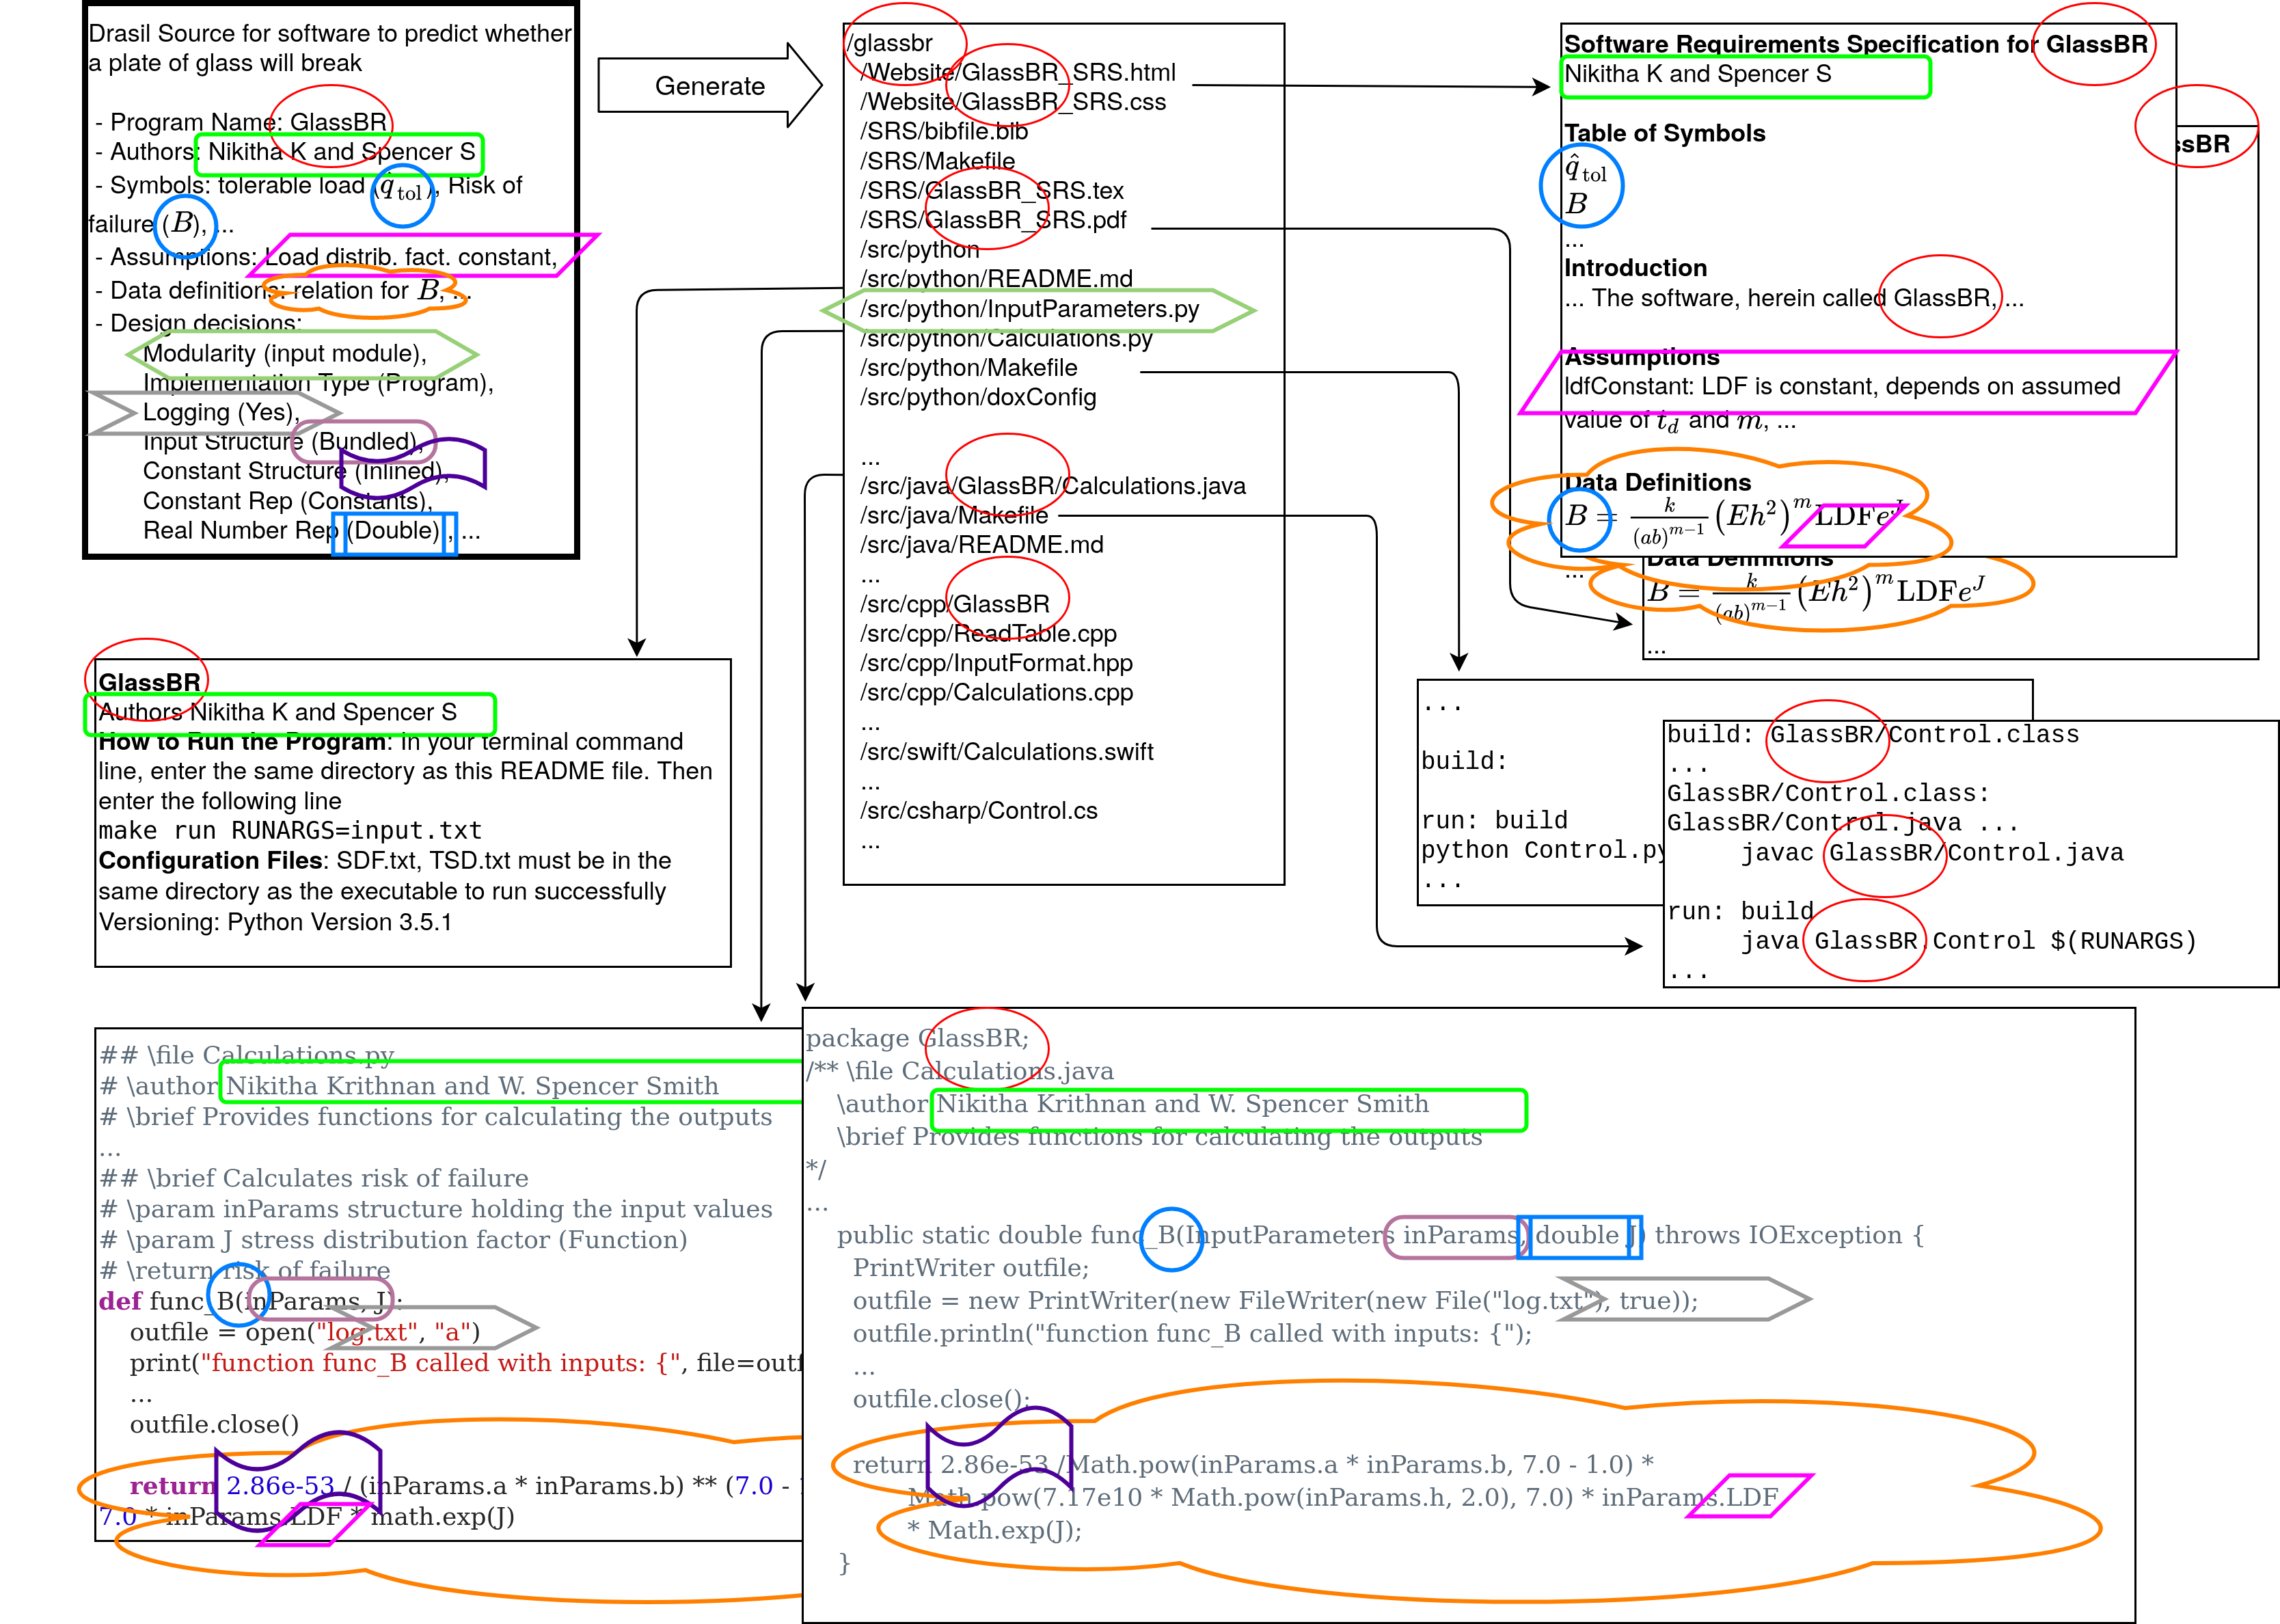
\includegraphics[width=0.75\textwidth]{assets/DrasilSupportsChange.png}
        \caption{Knowledge flow from ``knowledge-base''/source to artifacts, by Dr. Spencer Smith}
        \label{fig:glassbr}
    \end{figure}
\end{frame}

\begin{frame}
    \frametitle{Which case studies currently generate code?}

    \begin{itemize}
        \item<1-> \textbf{GlassBR} - Predicting whether or not a glass slab is likely to resist a specified blast.
        \item<2-> \textbf{Proportional Derivative Controller (PDController)} - Examining the output of a ``Power Plant'' (Process Variable) over time.
        \item<3-> \textbf{SWHS without Phase Change Material (NoPCM)} - Modelling of a solar water heating system without phase change material, predicting temperatures and change in heat energy of water and the PCM over time.
        \item<4-> \textbf{Projectile} - Determining if a launched projectile hits a target, assuming no flight collisions.
    \end{itemize}
\end{frame}

\begin{frame}
    \frametitle{Why don't all case studies generate software artifacts?}
    \framesubtitle{Where will I be contributing?}

    \onslide<2->{After all,}
    \begin{itemize}
        \item<3-> They're all covered under ``well understood'' domains!
        \item<4-> The SRS documents are generated!\\
    \end{itemize}

    \onslide<5->{Generating view-only data (e.g., SRS documents) is considerably easier than generating artifacts that are ``evaluated'' in some way or another (e.g., compilation/interpretation/static analysis)}

    \onslide<6->{A few, notable, blocking problems:}
    \begin{itemize}
        \item<7-> Confidently generating usable software artifacts without strong type information places significant stress on developers, resulting in a higher likelihood of bugs in artifacts.
        \item<8-> Existing ``theories''/``*Models''\footnotemark[1] don't expose enough information. They must be enriched, so that we can better interact with, and understand them.
    \end{itemize}

    \footnotetext[1]{\tiny Terminology is currently being changed, but is not reflected in many documents yet.}
\end{frame}

\subsection{Goal \#1: Typed Expression Language}

\begin{frame}
    \frametitle{Goal \#1: Typed Expression Language}
    \framesubtitle{Problem Description}
    
    \begin{itemize}
        \item<2-> Ensure only admissible expressions are used in GOOL-supported languages, and that all expressions are coherent.
        \item<3-> We want to ease developer cognitive load when writing expressions, as they will need to ensure their expressions are coherent, or else a type error can occur at runtime.
    \end{itemize}
\end{frame}

\begin{frame}
    \frametitle{Goal \#1: Typed Expression Language}
    \framesubtitle{What makes up a ``good'' solution?}
    
    \begin{itemize}
        \item<2-> Catches, within reason, all possible scenarios where an expression goes awry.
        \item<3-> Allows GOOL code generator to also become typed!
        \item<4-> Add extra functionality to existing expression languages safely, allowing for new data types to be introduced.
        \item<5-> Adding type information to expressions shouldn't be a burden!
    \end{itemize}
\end{frame}

\begin{frame}
    \frametitle{Goal \#1: Typed Expression Language}
    \framesubtitle{Current Progression}
    
    \begin{itemize}
        \item<2-> Split core mathematical expression language (Expr) into 3 variants (Expr, ModelExpr, and CodeExpr)
            \begin{itemize}
                \item<3-> `Expr' is a discrete, directly computable language, expected to have a \emph{total} conversion into code (e.g., calculator).
                \item<4-> Created `ModelExpr', which contains all other kinds of expressions we might want to express, but won't necessarily be directly convertible into code. There are still a few operations left in ``Expr'' that need to be moved over, however.
                    \begin{itemize}
                        \item<5-> Theories that rely on discussion of terms only found ``ModelExpr'' may only have code generated for them if we have rich enough data (see goal \#2).
                    \end{itemize}
                \item<6-> ``CodeExpr'' is a clone of `Expr', with a few extra functionalities for GOOL.
                \item<7-> Created a typed tagless final\cite{Carette2009finally} smart constructor encoding for writing expressions in ``Expr'' (or, optionally, ModelExpr).
            \end{itemize}
    \end{itemize}
\end{frame}

\begin{frame}
    \frametitle{Goal \#1: Typed Expression Language}
    \framesubtitle{What are the next steps?}
    
    \begin{itemize}
        \item<2-> Continue moving inadmissible terms from ``Expr'' into ``ModelExpr''.
        \item<3-> Moving literals from ``Expr'' \& ``ModelExpr'' into their own small language, so that areas that want \emph{strictly} literals can also have stronger restrictions on allowed data.
        \item<4-> Adjusting containers to allow for expressions with a type variable.
        \item<5-> Adding the final type signatures, using Haskell GADT syntax.
    \end{itemize}
\end{frame}

\subsection{Goal \#2: Theory Discrimination -- ``ModelKinds''}

\begin{frame}
    \frametitle{Goal \#2: Theory Discrimination -- ``ModelKinds''}
    \framesubtitle{Problem Description}
    
    \begin{itemize}
        \item<2-> ``RelationConcepts'' were heavily used in both displaying expressions, and code generation. They are essentially ``Relation''s (``Expr''s) with a natural language description of them.
        \item<3-> ``RelationConcept''s don't contain enough information on their own to be a core component usable in general code generation.
        \item<4-> If the ``shape'' of the expressions are not uniform, then writing more ``interpreters''/``views''/code generators for them required difficult pattern analysis. It's also not a total-conversion.
    \end{itemize}
\end{frame}

\begin{frame}
    \frametitle{Goal \#2: Theory Discrimination -- ``ModelKinds''}
    \framesubtitle{What makes up a ``good'' solution?}
    
    \begin{itemize}
        \item<2-> A good solution involves making the ``Relation''s a ``view'' of a more data-rich specialized container for each kind of ``Theory''/``*Model''.
        \item<3-> ``ModelKinds''
        \item<4-> By constructing our final data views through ``more steps'' (e.g., with more depth), we obtain a better understanding of our ``theories'', allowing us to do more with them.
        \item<5-> We should be able to easily add extra ``ModelKind'' variants.
    \end{itemize}
\end{frame}

\begin{frame}
    \frametitle{Goal \#2: Theory Discrimination -- ``ModelKinds''}
    \framesubtitle{Current Progression}
    
    \begin{itemize}
        \item<2-> All ``RelationConcepts'' have been replaced, with one of:
            \begin{itemize}
                \item<3-> EquationalModels: ``QDefinition''s
                \item<4-> EquationalRealms: ``MultiDefn''s
                \item<5-> EquationalConstraints: ``ConstraintSet''s
                \item<6-> DEModels: ``RelationConcept''s
                \item<7-> OthModels: ``RelationConcept''s
            \end{itemize}
        \item<8-> Considerable number of ``theories''/``*Models'' have been restructured, but there are still many that are pending classification.
            \begin{itemize}
                \item<9-> Most are best to be done once we have a typed expression language (so that we can better handle expressions that involve collections of sorts), and the rest are differential equation-related models (primarily Dong's domain).
            \end{itemize}
    \end{itemize}
\end{frame}

\begin{frame}
    \frametitle{Goal \#2: Theory Discrimination -- ``ModelKinds''}
    \framesubtitle{What are the next steps?}
    
    \begin{itemize}
        \item<2-> Understanding what kinds of needs we have for ``collections'', pushing this information back into the typed expression language (once that is fully typed), and then creating model containers for these models.
        \item<3-> For the differential equation-related models, we will need to build appropriate models for each possible kind.
    \end{itemize}
\end{frame}

%%%%%%%%%%%%%%%%%%%%%%%%%%%%%%%%%%%%%%%%%%%%%%%%%%%%%%%%%%%%%%%%%%%%%%%%%%%%%%%
%% ACKNOWLEDGEMENTS
%%%%%%%%%%%%%%%%%%%%%%%%%%%%%%%%%%%%%%%%%%%%%%%%%%%%%%%%%%%%%%%%%%%%%%%%%%%%%%%

\begin{frame}
    \frametitle{Acknowledgements}

    \begin{itemize}
        \item<2-> Both goals are as designated by Dr. Carette, Dr. Smith, and past (and present) Drasil authors.
        \item<3-> ``ModelKinds'' is based on Dr. Carette's implementation.
    \end{itemize}
\end{frame}

%%%%%%%%%%%%%%%%%%%%%%%%%%%%%%%%%%%%%%%%%%%%%%%%%%%%%%%%%%%%%%%%%%%%%%%%%%%%%%%
%% A FINAL THANK YOU
%%%%%%%%%%%%%%%%%%%%%%%%%%%%%%%%%%%%%%%%%%%%%%%%%%%%%%%%%%%%%%%%%%%%%%%%%%%%%%%

\begin{frame}
    \center
    \huge{Fin.}\\
    \normalsize{Thank you!}
\end{frame}

%%%%%%%%%%%%%%%%%%%%%%%%%%%%%%%%%%%%%%%%%%%%%%%%%%%%%%%%%%%%%%%%%%%%%%%%%%%%%%%
%% REFERENCES
%%%%%%%%%%%%%%%%%%%%%%%%%%%%%%%%%%%%%%%%%%%%%%%%%%%%%%%%%%%%%%%%%%%%%%%%%%%%%%%

\section{References}

\begin{frame}[allowframebreaks]
    \frametitle{References}

    \bibliography{references}
    \bibliographystyle{apalike}
\end{frame}

\end{document}
